\ProvidesFile{Mds.tex}[Message Driven Systems]


\subsection{Message Driven Systems}
\label{section::MDS}

\subsubsection{Зачем все это?}

В предыдущем разделе мы обсудили как устроен блокирующий observer pattern.
Давайте я поясню, что это значит.
Пусть у нас есть код:
\begin{cppcode}
int x = 42;
Observable<int> out([&x] () { return x; }); // data binding
Observer<int> in(print, print); // actions binding
  
out.subscribe(&in); // print 42
  
x = 24;
out.notify();  // print 24
x = 42;
in.unsubscribe();
out.notify(); // does nothing
\end{cppcode}
Я хочу обратить внимание на строки~5 и~8.
Когда строчка~5 исполнилась и мы перешли на строчку~6, то порт \verb"in" уже исполнили свое действие \verb"onSubscribe".
То есть \verb"subscribe" ждет соответствующего observer-а, пока он не завершит обработку на своем порте.
Аналогично в строчке~8, когда мы перемещаемся к строке~9, то все observer-ы подписанные на \verb"out" уже выполнили свои действия \verb"onNotify".
То есть метод \verb"notify" ждет, пока все observer-ы подписанные на observable выполнят свою работу.
Поэтому данная имплементация и называется блокирующей.

Теперь возникает вопрос: <<а что такое не блокирующий observer?>>
Оказывается просто так неблокирующего ничего быть не может.
Действительно, если вы посмотрите на любую свою программу, она всегда идет сверху вниз и выполняет команды по-порядку.
Если у вас голая функция \verb"main", то сложно даже представить, что означает фраза <<неблокирующий вызов функции>>.
Банально в какой момент эта функция будет исполняться?
Куда она запишет свое значение?
Когда мы ее результат прочитаем?
Чтобы это все имело смысл, нам нужно иметь некую экосистему в рамках которой можно определить неблокирующие вызовы.
В качестве такой экосистемы как раз и подходит среда функционирующая на основе передачи сообщений или Message Driven Systems.

\subsubsection{Что такое Message Driven System}


В рамках Message Driven System определено понятие агента.
Это минимальная сущность функционирующая в системе.
Агенты такой системы имеют свои собственные почтовые ящики и умеют выполнять какую-то работу и посылать себе или друг другу новые сообщения.
В такой среде агент работает только, когда к нему в почтовый ящик что-то прилетело, если он пуст, то агент засыпает.
Так же есть система, которая преобразует нативные сигналы операционной системы в сообщения среды.
Это сделано для того, чтобы агенты могли реагировать на события операционной системы.
Графически такую среду можно изобразить так
\[
\xymatrix@R=5pt{
  {\text{Agent1}}&{}&{\text{Agent2}}&{}&{\text{Agent3}}&{}\\
  {
  \begin{tabular}{c}
  mail box\\
  \begin{tabular}{|c|c|c|}
  \hline
  {}&{}&{}\\
  \hline
  \end{tabular}
  \end{tabular}
  }\ar@/^10pt/[rr]\ar@/_25pt/[rrrr]&{}&{
    \begin{tabular}{c}
  mail box\\
  \begin{tabular}{|c|c|c|}
  \hline
  {}&{}&{}\\
  \hline
  \end{tabular}
  \end{tabular}
  }&{}&{
    \begin{tabular}{c}
  mail box\\
  \begin{tabular}{|c|c|c|}
  \hline
  {}&{}&{}\\
  \hline
  \end{tabular}
  \end{tabular}
  }\ar@/_10pt/[ll]&{}\\
  {}&{}&{}&{}&{\phantom{
\includegraphics[scale=0.2]{Figures/pechkin.jpg}}}&{}\\
  {}&{}&{}&{}&{\rule{-2em}{0em}\text{OS}\quad
\includegraphics[scale=0.2]{Figures/pechkin.jpg}}\ar@{-->}@/^10pt/[uu]\ar@{-->}@/^10pt/[uull]\ar@{-->}@/^10pt/[uullll]&{}\\
}
\]
Здесь в роли почтальона Печкина выступает система, которая перерабатывает сообщения операционной среды в сообщения экосистемы и посылает их нужным адресатам (обозначено пунктирными стрелками).
Сплошные стрелки -- это сообщения, которые агенты посылают друг другу.
Есть разные виды подобных сред с разными гарантиями на передачу сообщений.
Но я буду рассматривать только те, которые встречаются в рамках одной физической машины.
Для меня будет важно, что системы бывают с агентами двух видов: активными и пассивными.

\paragraph{MDS с активными агентами}

Напомню, что в компьютере работу совершают ядра процессора.
На уровне операционной системы есть понятие thread-а.
Это такая сущность, которая содержит работу для ядра процессора и все необходимые данные.
И можно думать, что операционная система подсоединяет thread к ядру процессора и/или отсоединяет.
Любой thread запускается с указанием стартовой функции, которая и будет описывать работу исполняемую на ядре.

В качестве примера Message Driven System-ы с активными агентами подходит операционная система Windows.
Оказывается, что все поведение ОС из коробки построено на сообщениях.
Все сигналы в приложение от операционной системы приходят в виде сообщений.
Обмен информацией между приложениями ведется с помощью сообщений.
Когда запускается очередное приложение в операционной системе, оно запускается на новом thread-е.
При этом на этом thread-е создается почтовый ящик для получения сообщений и требуется запустить event loop.
Event loop -- это цикл, который обрабатывает сообщения если они есть в почтовом ящике, а если ничего нет, то нужно уснуть.
Соответствующую картинку можно нарисовать так:
\[
\xymatrix@R=5pt{
  {\text{App1}}&{}&{\text{App2}}&{}&{\text{App3}}\\
  {
  \begin{tabular}{c}
  mail box\\
  \begin{tabular}{|c|c|c|}
  \hline
  {}&{}&{}\\
  \hline
  \end{tabular}
  \end{tabular}
  }
  \ar@(l,l)@{-->}[dd]
  &{}&{
  \begin{tabular}{c}
  mail box\\
  \begin{tabular}{|c|c|c|}
  \hline
  {}&{}&{}\\
  \hline
  \end{tabular}
  \end{tabular}
  }
  \ar@(l,l)@{-->}[dd]
  &{}&{
  \begin{tabular}{c}
  mail box\\
  \begin{tabular}{|c|c|c|}
  \hline
  {}&{}&{}\\
  \hline
  \end{tabular}
  \end{tabular}
  }
  \ar@(l,l)@{-->}[dd]
  \\
  {
  {\text{Thread1}}
  }&{}&{
  {\text{Thread2}}
  }&{}&{
  {\text{Thread3}}
  }\\
  {
  {\text{event loop}}
  }
  \ar@(r, r)[uu]\ar@(r, l)[uurr]
  &{}&{
  {\text{event loop}}
  }
  \ar@(r, l)[uurr]
  &{}&{
  {\text{event loop}}
  }
  \ar@(r, r)[uu]
  \\
  {}&{}&{}&{}&{}\\
}
\]
Здесь каждый агент -- это отдельное приложение, которое имеет свой почтовый ящик и крутит на своем thread-е event loop.
Для полноты картины напишу как приблизительно выглядит event loop
\begin{cppcode}
int runEventLoop() {
  CMessageStatus Status;
  MSG CurrentMessage;
  while ((Status = ::GetMessage(&CurrentMessage, hwnd(), 0, 0)) != Quit) {
    if (Status == Error)
      handleError(&CurrentMessage);
    else
      ::TranslateMessage(CurrentMessage);
      ::DispatchMessage(CurrentMessage);
  }
  return exitCode(&CurrentMessage);
}
\end{cppcode}
Надо сказать, что перед запуском такого цикла обязательно должна быть команды создающие почтовый ящик, регистрирующие этот почтовый ящик в системе и прочие детали для внедрения в среду Windows.
Я весь этот код игнорирую.
Но давайте поймем  логическую структуру данного цикла.
В самом начале у нас есть две переменные для статуса и для сообщения.
Внутри \verb"while" цикла мы считываем текущее сообщение и записываем его статус в переменную \verb"Status".
Далее если статус это \verb"Quit", то мы выходим из цикла и программа завершается.
Если функция \verb"GetMessage" видит пустой ящик, то она усыпляет данный thread и цикл зависает.
Эта функциональность поддерживается автоматически из коробки.
Внутри цикла идет в начале обработчик ошибок.
А потом две стандартные функции, которые обеспечивают доставку сообщений в Windows.
Не спрашивайте меня почему их две, и почему у них такие дурацкие названия, это все следствие legacy.
Именно при вызове функции \verb"DispatchMessage" сообщение достается и отправляется в обработку.

\paragraph{MDS с пассивными агентами}
% TO DO

Примером Message Driven System-ы с пассивными агентами является экосистема Qt (читается cute).
На сегодняшний день это один из самых известных и мощных фреймворков для работы с GUI на C++.
Но как и C++, она максимально кривая и сложная для безопасного использования.
В рамках этой экосистемы выделяется один thread для event loop-а и на нем создается почтовый ящик.
Это все инкапсюлировано в объект \verb"QApplication".
Агентами в этой системе выступают \verb"QObject".
Это все возможные компоненты Qt графические и не только.
Например окно является агентом, кнопочка на нем является агентом, формы для ввода данных являются агентами и т.д.
Но все эти агенты не имеют своего thread-а для выполнения своих методов.
Вместо этого они лежат пассивно в памяти, а всю работу выполняет \verb"QApplicaion".
Думать про это надо так.
\verb"QApplication" -- это Папа Карло.
\verb"QObject"-ы -- это куча Буратин лежащих в комнате.
Что делает Папа Карло?
Во-первых, он ловит сообщения операционной системы и перерабатывает их в Qt сообщения и складывает в свой почтовый ящик.
Во-вторых, он вынимает из почтового ящика сообщения, смотри какая Буратина должна его получить.
Идет к этой буратине, и вызывает у него нужный метод.
В результате работы этого метода может быть появятся другие письма, которые будут сложены в почтовый ящик.
Давайте снабдим это описание картинкой.
\[
\xymatrix@C=15pt{
  {
  \begin{tabular}{c}
  {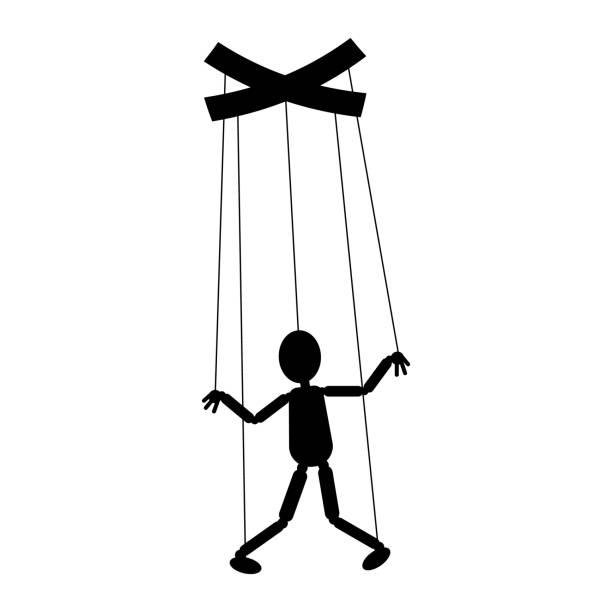
\includegraphics[scale=0.5]{Figures/marionette.jpg}}
  \\
  {\text{QObj1}}
  \end{tabular}
  }&{}&{
  \begin{tabular}{c}
  {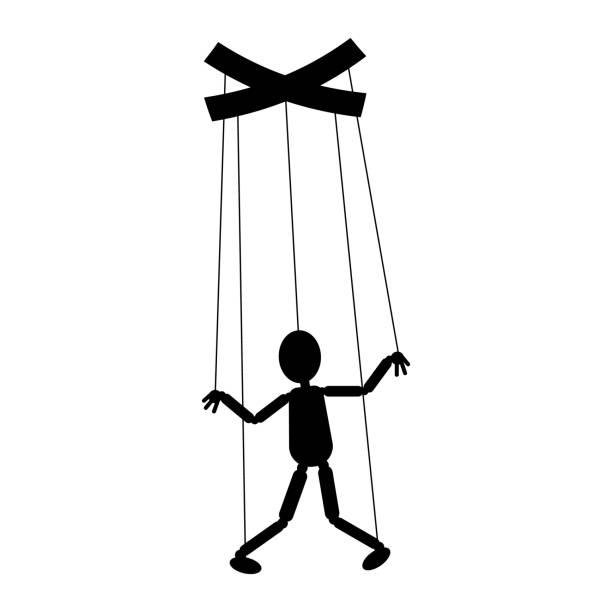
\includegraphics[scale=0.5]{Figures/marionette.jpg}}
  \\
  {\text{QObj2}}
  \end{tabular}
  }&{}&{
  \begin{tabular}{c}
  {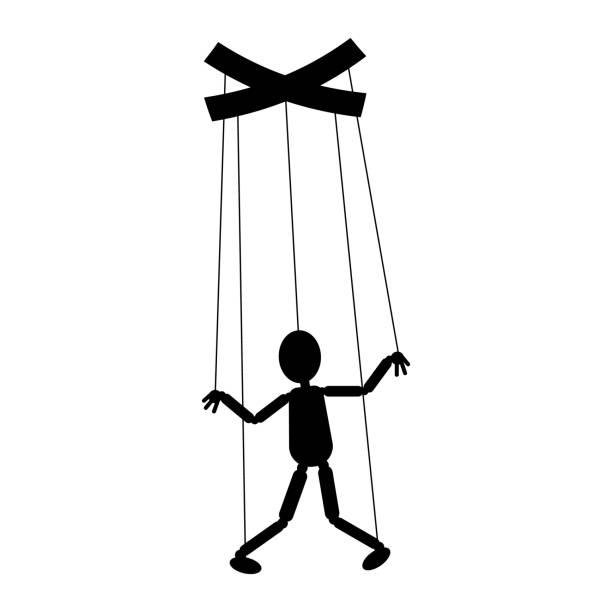
\includegraphics[scale=0.5]{Figures/marionette.jpg}}
  \\
  {\text{QObj3}}
  \end{tabular}
  }\\
  {
  \begin{tabular}{c}
  qApp\\
  Qt mail box\\
  \begin{tabular}{|c|c|c|}
  \hline
  {}&{}&{}\\
  \hline
  \end{tabular}\\
  {\textbf{Thread}}
  \end{tabular}
  }
  \ar@(r,r)[u]
  \ar@(r,d)[rru]
  \ar@(r,d)[rrrru]
  &{}&{}&{}&{
  {\textbf{OS}}
  }
  \ar@{-->}[llll]
  \\
}
\]
Так же для полноты картины давайте я приведу пример event loop в Qt экосистеме.
\begin{cppcode}
int main(int argc, char* argv[]) {
  QApplication QRunTime(argc, argv);
  Application application;
  QRunTime.exec();
  return 0;
}
\end{cppcode}
Вторая строчка создает Qt экосистему для данного thread-а.
Третья строчка создает объект приложения.
Важно, что его компоненты будут взаимодействовать с Qt экосистемой.
В этой строчке само приложение просто положили в память, корректно инициализировали и корректно подключили к Qt экосистеме.
И четвертая строчка запускает event loop.
Именно в этой функции крутится цикл, который выполняет всю работу.
В частности внутри этого цикла и будет выполняться работа при получении сообщения адресатом.

Функционирование Qt экосистемы можно представлять себе следующим образом:
\begin{center}
\begin{tabular}{rr}
{
1)\quad\scalebox{0.5}{
\boxed{
\begin{minipage}[\baselineskip]{12cm}
\[
\xymatrix@C=15pt{
  {}&{
  \begin{matrix}
  {\verb"QApplication"}\\
  {
  \begin{array}{|c|c|c|c|}
  \hline
  {\text{\color{red}\Letter}}&{\text{\Letter}}&{\ldots}&{\text{\Letter}}\\
  \hline
  \end{array}
  }
  %\ar@(l,u)[ld]
  %\ar@{<-}@(r,u)[rrdd]+(4,4)|-{\verb"postEvent"}
  \end{matrix}
  }&{}&{}\\
  {\phantom{\text{\Letter}}}
  %\ar[d]|-{\verb"event"}
  %\ar[dr]+(-4,15)|-{\verb"event"}
  %\ar[drrr]+(-4,15)|-{\verb"event"}&{}&{}&{}
  \\
  {
  \begin{matrix}
  {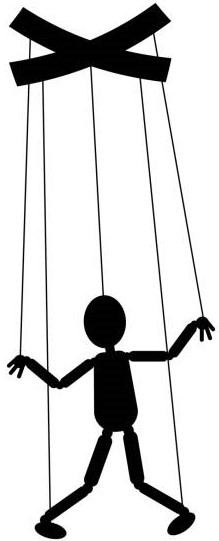
\includegraphics[scale=0.5]{Figures/marionette1.jpg}}\\
  {\verb"QObject1"}
  \end{matrix}
  }&{
  \begin{matrix}
  {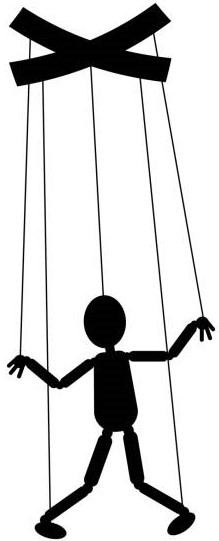
\includegraphics[scale=0.5]{Figures/marionette1.jpg}}\\
  {\verb"QObject2"}
  \end{matrix}
  }&{
  \begin{matrix}
  {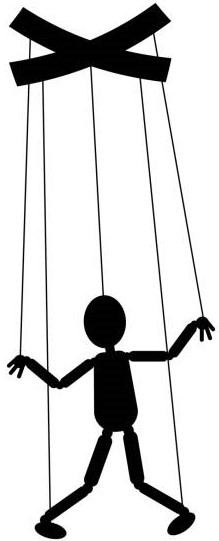
\includegraphics[scale=0.5]{Figures/marionette1.jpg}}\\
  {\verb"QObject3"}
  \end{matrix}
  }&{
  \begin{matrix}
  {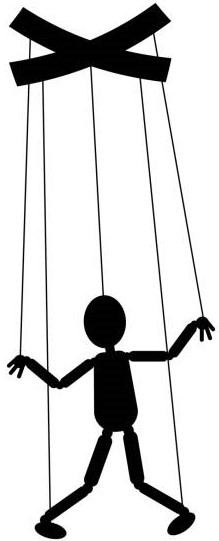
\includegraphics[scale=0.5]{Figures/marionette1.jpg}}\\
  {\verb"QObject4"}
  \end{matrix}
  }\\
}
\]
\end{minipage}
}}
}&{
5)\quad\scalebox{0.5}{
\boxed{
\begin{minipage}[\baselineskip]{12cm}
\[
\xymatrix@C=15pt{
  {}&{
  \begin{matrix}
  {\verb"QApplication"}\\
  {
  \begin{array}{|c|c|c|c|}
  \hline
  {\phantom{\text{\Letter}}}&{\text{\Letter}}&{\ldots}&{\text{\Letter}}\\
  \hline
  \end{array}
  }
  %\ar@(l,u)[ld]
  %\ar@{<-}@(r,u)[rrdd]+(4,4)|-{\verb"postEvent"}
  \end{matrix}
  }&{}&{}\\
  {{\text{\Letter}}}
  %\ar@[red][d]|-{\verb"event"}
  %\ar@[red][dr]+(-4,15)|-{\verb"event"}
  \ar@[red][drrr]+(-4,15)|-{\verb"event"}&{}&{}&{}
  \\
  {
  \begin{matrix}
  {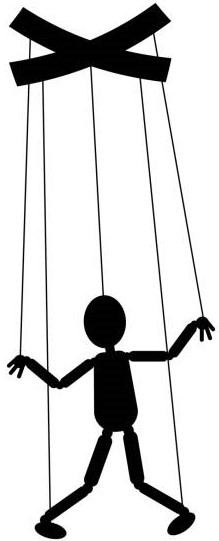
\includegraphics[scale=0.5]{Figures/marionette1.jpg}}\\
  {\verb"QObject1"}
  \end{matrix}
  }&{
  \begin{matrix}
  {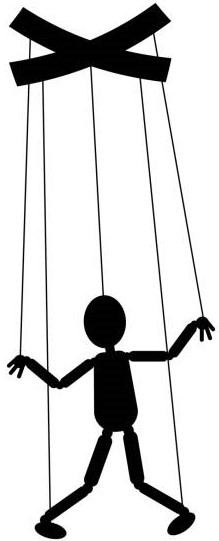
\includegraphics[scale=0.5]{Figures/marionette1.jpg}}\\
  {\verb"QObject2"}
  \end{matrix}
  }&{
  \begin{matrix}
  {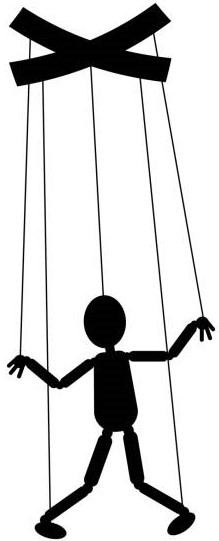
\includegraphics[scale=0.5]{Figures/marionette1.jpg}}\\
  {\verb"QObject3"}
  \end{matrix}
  }&{
  \begin{matrix}
  {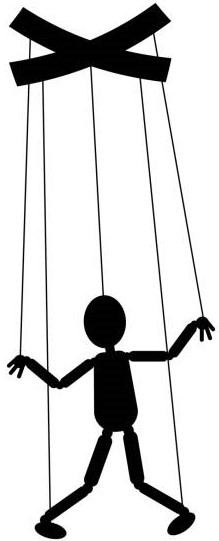
\includegraphics[scale=0.5]{Figures/marionette1.jpg}}\\
  {\verb"QObject4"}
  \end{matrix}
  }\\
}
\]
\end{minipage}
}}
}\\
{
2)\quad\scalebox{0.5}{
\boxed{
\begin{minipage}[\baselineskip]{12cm}
\[
\xymatrix@C=15pt{
  {}&{
  \begin{matrix}
  {\verb"QApplication"}\\
  {
  \begin{array}{|c|c|c|c|}
  \hline
  {\phantom{\text{\Letter}}}&{\text{\Letter}}&{\ldots}&{\text{\Letter}}\\
  \hline
  \end{array}
  }
  \ar@(l,u)[ld]
  %\ar@{<-}@(r,u)[rrdd]+(4,4)|-{\verb"postEvent"}
  \end{matrix}
  }&{}&{}\\
  {{\text{\color{red}\Letter}}}
  %\ar[d]|-{\verb"event"}
  %\ar[dr]+(-4,15)|-{\verb"event"}
  %\ar[drrr]+(-4,15)|-{\verb"event"}&{}&{}&{}
  \\
  {
  \begin{matrix}
  {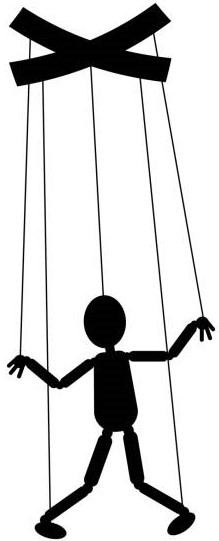
\includegraphics[scale=0.5]{Figures/marionette1.jpg}}\\
  {\verb"QObject1"}
  \end{matrix}
  }&{
  \begin{matrix}
  {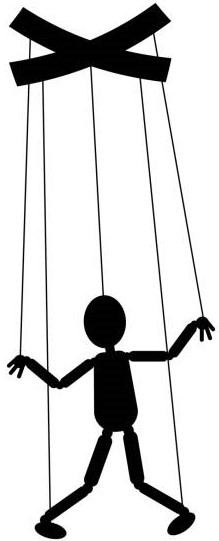
\includegraphics[scale=0.5]{Figures/marionette1.jpg}}\\
  {\verb"QObject2"}
  \end{matrix}
  }&{
  \begin{matrix}
  {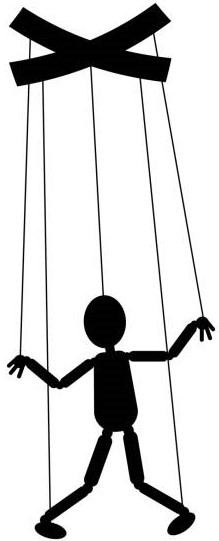
\includegraphics[scale=0.5]{Figures/marionette1.jpg}}\\
  {\verb"QObject3"}
  \end{matrix}
  }&{
  \begin{matrix}
  {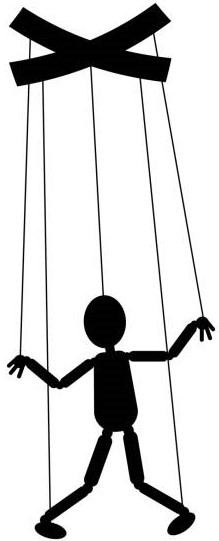
\includegraphics[scale=0.5]{Figures/marionette1.jpg}}\\
  {\verb"QObject4"}
  \end{matrix}
  }\\
}
\]
\end{minipage}
}}
}&{
6)\quad\scalebox{0.5}{
\boxed{
\begin{minipage}[\baselineskip]{12cm}
\[
\xymatrix@C=15pt{
  {}&{
  \begin{matrix}
  {\verb"QApplication"}\\
  {
  \begin{array}{|c|c|c|c|}
  \hline
  {\phantom{\text{\Letter}}}&{\text{\Letter}}&{\ldots}&{\text{\Letter}}\\
  \hline
  \end{array}
  }
  %\ar@(l,u)[ld]
  \ar@{<-}@(r,u)@[red][rrdd]+(4,4)|-{\verb"postEvent"}
  \end{matrix}
  }&{}&{}\\
  {{\text{\Letter}}}
  %\ar@[red][d]|-{\verb"event"}
  %\ar@[red][dr]+(-4,15)|-{\verb"event"}
  \ar[drrr]+(-4,15)|-{\verb"event"}&{}&{}&{}
  \\
  {
  \begin{matrix}
  {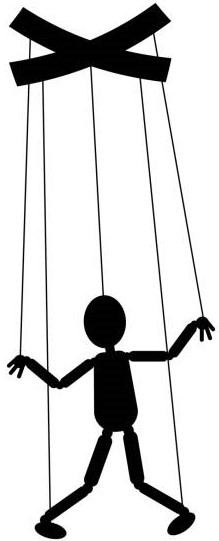
\includegraphics[scale=0.5]{Figures/marionette1.jpg}}\\
  {\verb"QObject1"}
  \end{matrix}
  }&{
  \begin{matrix}
  {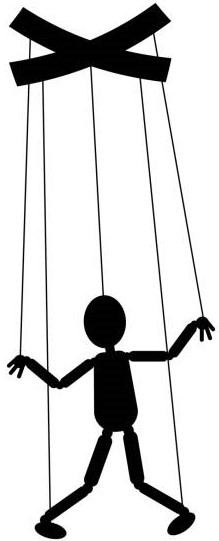
\includegraphics[scale=0.5]{Figures/marionette1.jpg}}\\
  {\verb"QObject2"}
  \end{matrix}
  }&{
  \begin{matrix}
  {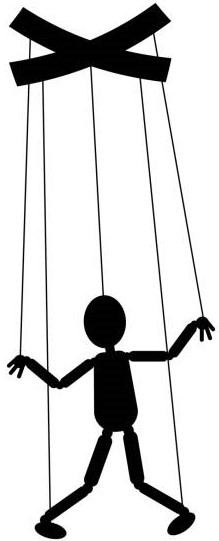
\includegraphics[scale=0.5]{Figures/marionette1.jpg}}\\
  {\verb"QObject3"}
  \end{matrix}
  }&{
  \begin{matrix}
  {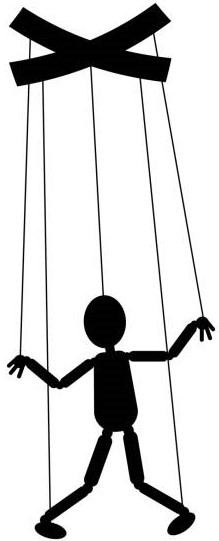
\includegraphics[scale=0.5]{Figures/marionette1.jpg}}\\
  {\verb"QObject4"}
  \end{matrix}
  }\\
}
\]
\end{minipage}
}}
}\\
{
3)\quad\scalebox{0.5}{
\boxed{
\begin{minipage}[\baselineskip]{12cm}
\[
\xymatrix@C=15pt{
  {}&{
  \begin{matrix}
  {\verb"QApplication"}\\
  {
  \begin{array}{|c|c|c|c|}
  \hline
  {\phantom{\text{\Letter}}}&{\text{\Letter}}&{\ldots}&{\text{\Letter}}\\
  \hline
  \end{array}
  }
  %\ar@(l,u)[ld]
  %\ar@{<-}@(r,u)[rrdd]+(4,4)|-{\verb"postEvent"}
  \end{matrix}
  }&{}&{}\\
  {{\text{\Letter}}}
  \ar@[red][d]|-{\verb"event"}
  %\ar[dr]+(-4,15)|-{\verb"event"}
  %\ar[drrr]+(-4,15)|-{\verb"event"}&{}&{}&{}
  \\
  {
  \begin{matrix}
  {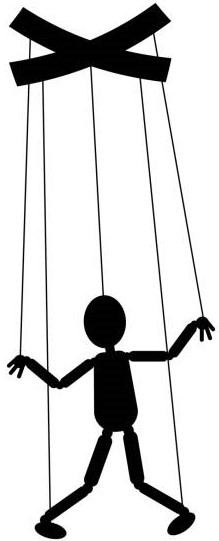
\includegraphics[scale=0.5]{Figures/marionette1.jpg}}\\
  {\verb"QObject1"}
  \end{matrix}
  }&{
  \begin{matrix}
  {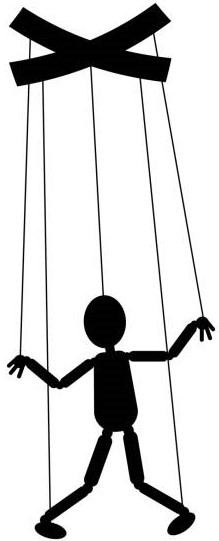
\includegraphics[scale=0.5]{Figures/marionette1.jpg}}\\
  {\verb"QObject2"}
  \end{matrix}
  }&{
  \begin{matrix}
  {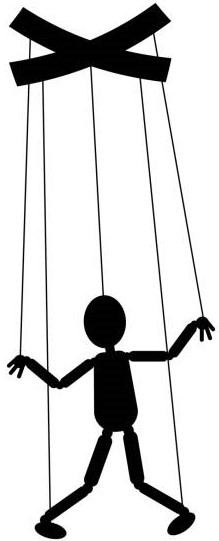
\includegraphics[scale=0.5]{Figures/marionette1.jpg}}\\
  {\verb"QObject3"}
  \end{matrix}
  }&{
  \begin{matrix}
  {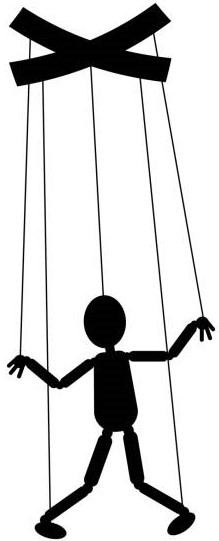
\includegraphics[scale=0.5]{Figures/marionette1.jpg}}\\
  {\verb"QObject4"}
  \end{matrix}
  }\\
}
\]
\end{minipage}
}}
}&{
7)\quad\scalebox{0.5}{
\boxed{
\begin{minipage}[\baselineskip]{12cm}
\[
\xymatrix@C=15pt{
  {}&{
  \begin{matrix}
  {\verb"QApplication"}\\
  {
  \begin{array}{|c|c|c|c|}
  \hline
  {{\text{\Letter}}}&{\text{\Letter}}&{\ldots}&{\text{\color{red}\Letter}}\\
  \hline
  \end{array}
  }
  %\ar@(l,u)[ld]
  \ar@{<-}@(r,u)[rrdd]+(4,4)|-{\verb"postEvent"}
  \end{matrix}
  }&{}&{}\\
  {{\text{\Letter}}}
  %\ar@[red][d]|-{\verb"event"}
  %\ar@[red][dr]+(-4,15)|-{\verb"event"}
  \ar[drrr]+(-4,15)|-{\verb"event"}&{}&{}&{}
  \\
  {
  \begin{matrix}
  {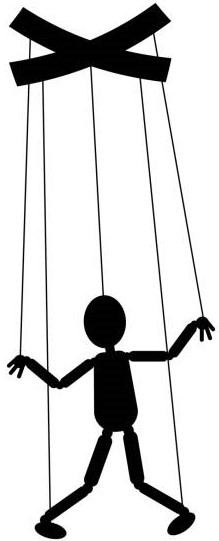
\includegraphics[scale=0.5]{Figures/marionette1.jpg}}\\
  {\verb"QObject1"}
  \end{matrix}
  }&{
  \begin{matrix}
  {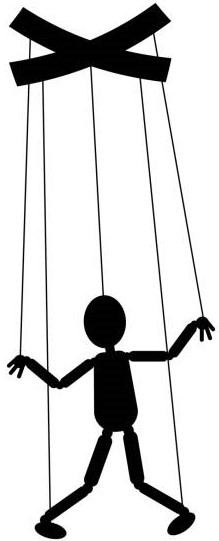
\includegraphics[scale=0.5]{Figures/marionette1.jpg}}\\
  {\verb"QObject2"}
  \end{matrix}
  }&{
  \begin{matrix}
  {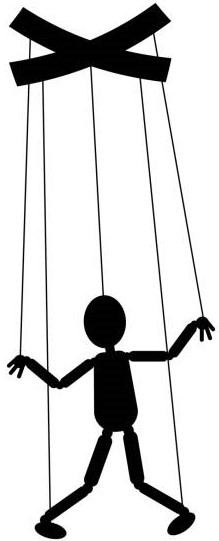
\includegraphics[scale=0.5]{Figures/marionette1.jpg}}\\
  {\verb"QObject3"}
  \end{matrix}
  }&{
  \begin{matrix}
  {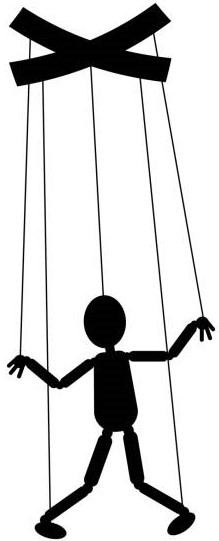
\includegraphics[scale=0.5]{Figures/marionette1.jpg}}\\
  {\verb"QObject4"}
  \end{matrix}
  }\\
}
\]
\end{minipage}
}}
}\\
{
4)\quad\scalebox{0.5}{
\boxed{
\begin{minipage}[\baselineskip]{12cm}
\[
\xymatrix@C=15pt{
  {}&{
  \begin{matrix}
  {\verb"QApplication"}\\
  {
  \begin{array}{|c|c|c|c|}
  \hline
  {\phantom{\text{\Letter}}}&{\text{\Letter}}&{\ldots}&{\text{\Letter}}\\
  \hline
  \end{array}
  }
  %\ar@(l,u)[ld]
  %\ar@{<-}@(r,u)[rrdd]+(4,4)|-{\verb"postEvent"}
  \end{matrix}
  }&{}&{}\\
  {{\text{\Letter}}}
  %\ar@[red][d]|-{\verb"event"}
  \ar@[red][dr]+(-4,15)|-{\verb"event"}
  %\ar[drrr]+(-4,15)|-{\verb"event"}&{}&{}&{}
  \\
  {
  \begin{matrix}
  {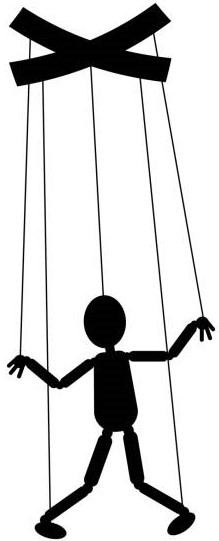
\includegraphics[scale=0.5]{Figures/marionette1.jpg}}\\
  {\verb"QObject1"}
  \end{matrix}
  }&{
  \begin{matrix}
  {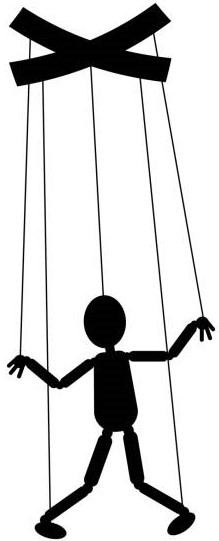
\includegraphics[scale=0.5]{Figures/marionette1.jpg}}\\
  {\verb"QObject2"}
  \end{matrix}
  }&{
  \begin{matrix}
  {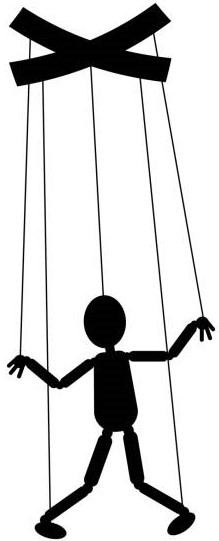
\includegraphics[scale=0.5]{Figures/marionette1.jpg}}\\
  {\verb"QObject3"}
  \end{matrix}
  }&{
  \begin{matrix}
  {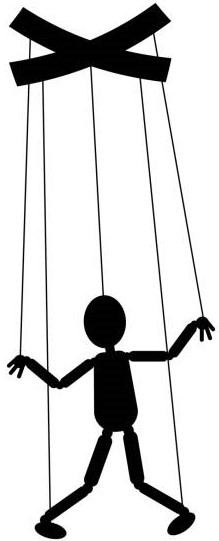
\includegraphics[scale=0.5]{Figures/marionette1.jpg}}\\
  {\verb"QObject4"}
  \end{matrix}
  }\\
}
\]
\end{minipage}
}}
}&{
}\\
\end{tabular}
\end{center}
Прокомментируем поведение системы выше:
\begin{enumerate}
\item \verb"QApplication" проверяет пуст ли почтовый ящик или нет.
Если почтовый ящик пуст, то система засыпает пока не появятся сообщения от операционной системы.
Эти сообщения будут трансформированы в Qt сообщения и сложены в почтовый ящик.

\item Если почтовый ящик не пуст, то вынимаем первое сообщение из ящика.
Теперь можно совершать доставку сообщения адресатам

\item В Qt экосистеме обработчик сообщения у адресата -- функция \verb"event".
Вызываем эту функцию для \verb"QObject1" и передаем в нее текущее сообщение.

\item Теперь вызываем \verb"event" у \verb"QObject2" и передаем в нее текущее сообщение.

\item На этом шаге вызываем \verb"event" у \verb"QObject4" и передаем в нее текущее сообщение.

\item В результате обработки сообщения \verb"QObject4" сформировал сообщение и отправляет его в почтовый ящик \verb"QApplication".

\item Сообщение от \verb"QObject4" положили в конец очереди в почтовый ящик.
На этом одна итерация event loop-а завершается и весь процесс повторяется с самого начала.
\end{enumerate}


\subsubsection{Идея имплементации}

Я уже приводил пример event loop-а для двух Message Driven System.
Давайте я в общих чертах скажу, как строится произвольная такая система.
Прежде всего у нас должен почтовый ящик и event loop, которые выглядят как-то так.
\begin{cppcode}
MailBox gBox;

int main() {
  Event e;
  while(getEvent(&e)) {
    dispatchEvent(e);
  }
  return 0;
}
\end{cppcode}
Тут важно понимать, что почтовый ящик является глобальным ресурсом для данного thread-а.
Как мы видим весь event loop устроен очень просто, мы вынимаем сообщение из почтового ящика в функции \verb"getEvent".
А потом запускаем доставку сообщений в методе \verb"dispatchEvent".
При такой имплементации цикл заканчивается, если \verb"getEvent" вернет \verb"false".
В этой имплементации отсутствует код, перерабатывающий сообщения операционной системы в сообщения экосистемы.

Функция доставки сообщений работает приблизительно так
\begin{cppcode}
void dispatchEvent(const Event& e) {
  for (auto obj : addresseesOf(e)) {
    obj->handleEvent(e);
  }
}
\end{cppcode}
То есть для каждого сообщения составляется список его адресатов, а потом мы просто зовем служебную функцию \verb"handleEvent" у всех адресатов блокирующим образом.

Теперь, что из себя представляет сообщение?
Обычно это данные и некоторая метаинформация, которая помогает понять, что это за данные.
Ведь передавать мы должны уметь все что угодно.
Кратко можно думать про это так
\begin{cppcode}
enum class EventType {
  Mouse,
  Keyboard,
  /* ... */};

class Event {
public:
  /*Constructor*/
  EventType type() const;
  const void* data() const;
  
private:
  EventType type_;
  std::any data_;
};
\end{cppcode}
Здесь \verb"EventType" -- это заранее известный набор констант для всех возможных типов сообщений.
Многие системы имеют выделенный диапазон типов для создания пользовательских сообщений.
Само сообщение содержит информацию о типе и данные.
Я использую \verb"std::any" как стирающий тип, который умеет хранить что угодно.

Теперь перейдем к обработке сообщений.
Для хранения списка адресатов, который используется в функции \verb"dispatchEvent" можно использовать интерфейсы или стирающие ссылки.
\begin{cppcode}
std::vector<EventHandler> addresseesOf(const Event& e)
\end{cppcode}
здесь \verb"EventHandler" -- это стирающий указатель на объект, которому доставляется сообщение.
Для попадания в этот список в системе должны быть свои механизмы, которые я тут не собираюсь обсуждать.
Теперь обработка сообщений выглядит как-то так
\begin{cppcode}
class Obj1 {
public:
  void handleEvent(const Event& e) override {
    switch(e.type()) {
      case EventType::Mouse:
        MouseEvent& Data = cast<MouseEvent&>(e.data());
        // handle mouse event
      break;
      case EventType::Keyboard:
        KeyboardEvent& Data = cast<KeyboardEvent&>(e.data());
        // handle keyboard event
      break;
      ...
    }
  }
};
\end{cppcode}
Каждый объект должен прочитать тип сообщения, а потом в зависимости от этой информации вынуть нужные данные и отреагировать на них.
Возможно, что \verb"handleEvent" игнорирует какие-то сообщения, а может быть даже и все.
Функция \verb"cast" выше -- это псевдокод, который призван показать, что мы вынимаем из сообщения данные, которые там зашифрованы в зависимости от информации о типе сообщения.

\subsubsection{Неблокирующие операции}
% TO DO

Теперь, если мы орудуем в рамках Message Driven System, у нас есть два способа отправить данные из одной функции в другую.
\begin{enumerate}
\item Прямой блокирующий вызов.
Этот случай -- это просто обычный вызов функции внутри другой функции.
Например, если работает обработчик сообщений \verb"Obj1", то он может дернуть (если знает адрес) какой-нибудь метод из \verb"Obj2".
В этом случае реакция на данные происходит немедленно.

\item Посылка сообщения.
В этом случае если обработчик сообщений \verb"Obj1" произвел какие-то данные для \verb"Obj2", то он не вызывает метод \verb"Obj2".
Вместо этого он создает сообщение, куда складывает эту информацию, пишет в качестве адресата \verb"Obj2" на конверте и складывает письмо в почтовый ящик.
В этом случае реакция на сообщение произойдет не сразу же во время отправки сообщения, а позже, когда экосистема дойдет до обработки сообщения и передаст его адресату.
Такое поведение называется неблокирующим вызовом.
Это поведение важно держать в голове, потому что важно поместить в сообщение все данные, чтобы они были живы, когда сообщение дойдет до адресата.
Нельзя вкладывать ссылки и указатели на локальные данные, просто потому что они все умрут к моменту передачи сообщения по назначению.
\end{enumerate}
Второй подход нужен для того, чтобы не блокировать на долго одной задачей ядро процессора.
Чтобы на одном ядре успевали покрутиться разные обработчики сообщений.
Это делается для того, чтобы GUI был отзывчивым и окна не подвисали.
В рамках такой экосистемы полезно иметь неблокирующий observer pattern, в котором observable не сразу дергает методы \verb"onSubscribe" и \verb"onNotify", а посылает сообщения через Message Driven System.
